\documentclass[11pt]{article}

\usepackage[margin=1in]{geometry}
\usepackage{booktabs}
\usepackage{graphicx}
\usepackage{hyperref}
\usepackage[most]{tcolorbox}

\newtcolorbox{modelquote}[1]{
  colback=blue!5,
  colframe=blue!35,
  title=#1,
  fonttitle=\bfseries,
  arc=1mm,
  boxrule=0.6pt,
  left=6pt,
  right=6pt,
  top=6pt,
  bottom=6pt
}

\title{A Pilot LLM Replication of Clark and Wilkes-Gibbs' Tangram Task}
\author{}
\date{}

\begin{document}
\maketitle

\section*{Overview}

Clark and Wilkes-Gibbs (1986) showed that pairs of human participants rapidly converge on concise referring expressions when they repeatedly collaborate on a Tangram arrangement task. In the original study, a director and matcher had the same 12 abstract Tangram figures in different orders. The director's task was to get the matcher to rearrange their figures into the director's order, proceeding through positions 1--12. The same pair repeated the task for six trials. The central finding was a large reduction in director words and turns per figure across trials, accompanied by very high accuracy.

We ran a first pilot version of the same task using Claude Haiku 4.5 as both director and matcher. We then ran the same setup with GPT-5.5 at \texttt{xhigh} reasoning effort. The instructions were intentionally minimal: the models were told the task situation, the hidden-arrangement constraint, the 1--12 ordering procedure, and the required text-interface actions. We did not instruct the models to use particular descriptive strategies, to be tentative, to compare figures, or to ask clarifying questions. Thus, the run was designed as a close text-only analogue of the paper's task constraints rather than an optimized prompt for model performance.

This report summarizes one complete Haiku pair over six trials and one complete GPT-5.5 pair over six trials. It should be treated as a pilot, not as an inferential comparison to the full human sample of eight pairs.

\section*{Method}

The first model was \texttt{claude-haiku-4-5-20251001}. The second model was \texttt{gpt-5.5} with \texttt{xhigh} reasoning effort. Both roles retained the full prior dialogue across trials, as in the human repeated-reference design. The 12 Tangram figures were shown as separate images. Internal figure labels were used only for scoring and were not presented as shared labels. Each participant had private image numbers, independently randomized, and these were not valid communicative references.

Both runs used the same minimal paper-style instruction set. The Haiku and GPT-5.5 runs both terminated normally for all six trials.

\section*{Primary Results}

\subsection*{Model comparison}

The main quantitative contrast is stark. GPT-5.5 placed every figure correctly for the first five trials and made four errors in trial 6, for 68/72 correct placements overall. Haiku was well above a random baseline but much less accurate. GPT-5.5 also used many fewer director words per figure than Haiku, but it did not reproduce the human pattern of strong progressive shortening.

\begin{table}[h]
\centering
\begin{tabular}{lrrrr}
\toprule
Run & Trials included & Accuracy & Words/figure & Turns/figure \\
\midrule
Human paper & 6 & $\sim$.98 & $\sim$16.8 & $\sim$1.77 \\
Haiku 4.5 & 6 & .444 & 107.76 & 1.10 \\
GPT-5.5 xhigh & 6 & .944 & 50.31 & 1.00 \\
\bottomrule
\end{tabular}
\caption{Headline comparison. The human row uses the published approximate 2\% error rate and the mean of the published words- and turns-per-figure values across the six trials.}
\end{table}

\subsection*{Words per figure}

The strongest contrast with the human data is in the word-count trajectory. Human directors in Clark and Wilkes-Gibbs showed a steep reduction from about 41 words per figure on trial 1 to about 8 by trial 6. Haiku did not show this shortening. Its director produced a little over 100 words per figure on every trial. GPT-5.5 was much more concise than Haiku, but it also did not show human-like compression: it stayed near 50 words per figure across the six trials.

\begin{table}[h]
\centering
\resizebox{\linewidth}{!}{%
\begin{tabular}{rrrrrr}
\toprule
Trial & Haiku words/figure & GPT-5.5 words/figure & Human words/figure & Haiku correct & GPT correct \\
\midrule
1 & 107.50 & 54.25 & 41 & 5/12 & 12/12 \\
2 & 109.33 & 51.67 & 19 & 6/12 & 12/12 \\
3 & 107.42 & 49.25 & 13 & 5/12 & 12/12 \\
4 & 108.50 & 48.75 & 11 & 6/12 & 12/12 \\
5 & 107.25 & 48.75 & 9 & 4/12 & 12/12 \\
6 & 106.58 & 49.17 & 8 & 6/12 & 8/12 \\
\bottomrule
\end{tabular}
}
\caption{Words per figure and accuracy by trial. Human values are the published approximate means from Clark and Wilkes-Gibbs.}
\end{table}

\begin{figure}[h]
\centering
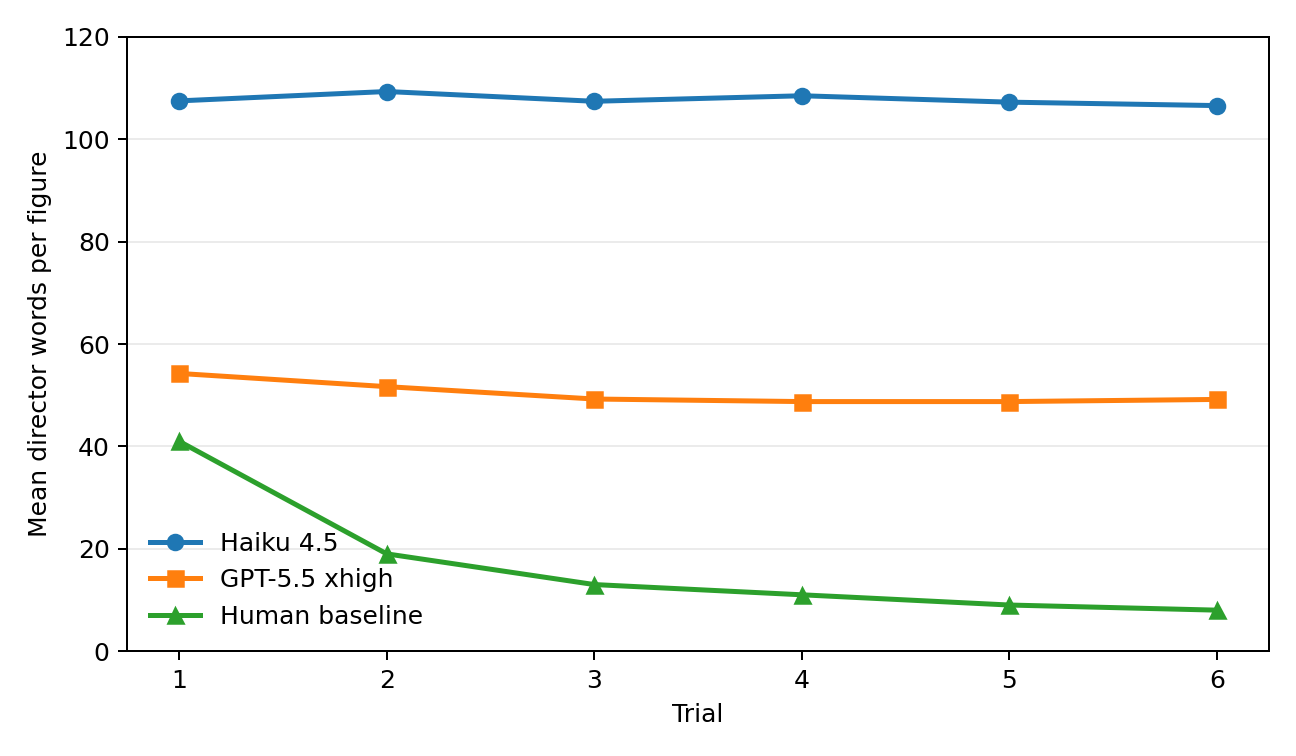
\includegraphics[width=0.72\linewidth]{report_figures/model_words_per_trial.png}
\caption{Words per figure by trial.}
\end{figure}

\subsection*{Turns per figure}

Human directors also reduced their turns per figure across trials, from about 3.7 to about 1.2. Both model pairs used about one director turn per figure throughout. This is not the same pattern as the human data. Rather than converging from initially extended negotiation to later concise exchanges, the models generally offered a description and the matcher placed a figure quickly.

\begin{table}[h]
\centering
\begin{tabular}{rrrr}
\toprule
Trial & Haiku director turns/figure & GPT director turns/figure & Human director turns/figure \\
\midrule
1 & 1.17 & 1.00 & 3.7 \\
2 & 1.08 & 1.00 & 1.9 \\
3 & 1.08 & 1.00 & 1.4 \\
4 & 1.08 & 1.00 & 1.3 \\
5 & 1.08 & 1.00 & 1.1 \\
6 & 1.08 & 1.00 & 1.2 \\
\bottomrule
\end{tabular}
\caption{Mean director turns per figure.}
\end{table}

\subsection*{Accuracy}

The original human error rate was about 2\%. Haiku's accuracy was much lower and did not improve across trials. Across the six trials, Haiku placed 32 of 72 figures correctly, for an overall accuracy of 44.4\%. GPT-5.5 placed 68 of 72 figures correctly, for 94.4\% accuracy. Its errors were concentrated in the final trial, where two pairs of figures were swapped: K/L and A/E.

Haiku's result, though low, is well above a random-ordering baseline. For a random permutation of 12 figures, the expected number of correct positions is 1 per trial, or 6 correct placements over six trials. Under the exact random-permutation distribution, obtaining 32 or more correct placements out of 72 has probability approximately $9.1 \times 10^{-14}$. Thus, Haiku was not guessing: it extracted useful information from the images and dialogue, but did so much less effectively than human participants.

\subsection*{Basic exchanges}

In the human data, basic exchanges increased from 18\% on trial 1 to over 80\% by trials 4--6. Haiku's exchanges were basic in a different and less successful sense. After trial 1, nearly every placement had the director present a reference and the matcher place a figure in the first response, but this co-occurred with low accuracy, suggesting premature acceptance rather than well-established shared reference. GPT-5.5 also used one-step placements, but these were usually accurate until the final-trial swaps.

\subsection*{Position effects}

Clark and Wilkes-Gibbs reported that, within a trial, later positions required fewer words because fewer candidate figures remained. This slope weakened across trials. Haiku did not show the same pattern. In this pilot, the estimated Haiku slope of words by position was approximately $-0.42$ in trial 1, $+3.85$ in trial 2, and $+2.79$ in trial 6. GPT-5.5 also showed little evidence of the human-like within-trial economy, with corresponding slopes of approximately $+1.06$, $+0.44$, and $-0.20$. These values are not comparable to the human slope pattern of roughly $-4.6$, $-1.0$, and $-0.4$ for trials 1, 2, and 6 respectively.

\subsection*{Figure-level difficulty}

The paper reported figure-level differences, with Figure B hardest and Figure C easiest by word count. In the Haiku pilot, word count and accuracy were not tightly aligned. Figure B was again among the most verbally costly and was never placed correctly, but Figure J was also highly verbose while being placed correctly in every trial.

\begin{table}[h]
\centering
\resizebox{\linewidth}{!}{%
\begin{tabular}{rrrrrr}
\toprule
Figure & Haiku words/figure & Haiku accuracy & GPT words/figure & GPT accuracy & GPT label \\
\midrule
A & 86.83 & .000 & 49.17 & .833 & tall standing two-top-pieces \\
B & 138.67 & .000 & 50.67 & 1.000 & dancer/bird \\
C & 94.83 & .167 & 49.33 & 1.000 & long diagonal flying \\
D & 114.67 & .167 & 53.33 & 1.000 & tall upright / left shelf \\
E & 132.67 & .167 & 50.33 & .833 & reclining shoe/lounging animal \\
F & 110.00 & .833 & 52.00 & 1.000 & low crouching \\
G & 118.33 & .833 & 56.00 & 1.000 & low long flat-base figure \\
H & 86.33 & .667 & 41.17 & 1.000 & bottle/vase-shaped \\
I & 90.00 & .667 & 54.67 & 1.000 & right-facing animal / left protrusion \\
J & 134.50 & 1.000 & 51.33 & 1.000 & compact upright blocky \\
K & 102.67 & .667 & 48.33 & .833 & upright zigzag / beak-arm \\
L & 83.67 & .167 & 47.33 & .833 & tall zigzag leg/foot \\
\bottomrule
\end{tabular}
}
\caption{Figure-level results. Both model rows use six trials. GPT labels summarize recurring director expressions.}
\end{table}

\section*{Qualitative Impression}

The transcripts suggest that Haiku understood the formal mechanics of the task but did not develop efficient shared referring expressions. The director often produced long, generic descriptions using recurring terms such as diamond head, angular body, pointed extensions, or geometric figure. These descriptions were plausible but insufficiently discriminating among the 12 similar figures. The matcher frequently accepted and placed a figure immediately, even when the description could apply to several candidates. This produced a superficially efficient exchange structure but poor task success.

In the human study, reduced word and turn counts reflected successful convergence on mutually accepted perspectives. In the Haiku pilot, low turn counts appear to reflect premature placement rather than mutual understanding. The model did not show the central Clark and Wilkes-Gibbs pattern: repeated collaboration did not yield shorter, stable, successful referring expressions.

\begin{modelquote}{Haiku example: generic geometric description}
\emph{``This figure has a rotated square at the top, and below it is a larger angular shape that extends downward and slightly to the right. The body is more jagged and irregular compared to position 2, with a pointed or angular bottom section.''}
\end{modelquote}

GPT-5.5 behaved differently. Its first-trial descriptions were still detailed, but they were organized around distinctive, image-specific visual anchors. The director combined overall silhouette, head type and location, distinctive appendages, and base or foot shape. Examples include \emph{long diagonal flying}, \emph{low crouching}, \emph{upright zigzag}, \emph{bottle/vase-shaped}, \emph{left-pointing triangular protrusion}, \emph{flat base}, and \emph{right-pointing beak/arm}. These expressions were sufficiently discriminating for the matcher to identify the intended figure on the first placement attempt through the first five trials.

\begin{modelquote}{GPT-5.5 example: distinctive visual anchors}
\emph{``Position 2: the long diagonal `flying' one. It has a small tilted square sitting near the upper middle-left, a broad flat wing/arm sticking out to the left.''}
\end{modelquote}

By trial 2, GPT-5.5 was already reusing shared references established in the prior dialogue. Its dominant device was to combine a previous-trial position reference with a brief visual label, for example ``the same figure that was position 9 in the previous trial'' plus ``the low crouching animal-like one''. This resembles the qualitative direction of the human findings: the pair used prior common ground to support later reference. The difference is that GPT-5.5 achieved high accuracy almost immediately, with relatively little negotiation, rather than gradually constructing these conventions through many repair sequences.

\begin{modelquote}{GPT-5.5 example: reuse of shared labels}
\emph{``Trial 5, position 1: use the same figure that was position 5 in the previous trial -- the bottle/vase-shaped vertical figure with a diamond head on top.''}
\end{modelquote}

The final trial shows a limitation of this strategy. GPT-5.5's four errors were not random scatter; they were two swaps among visually related figures. It confused K with L after both had been described with zigzag/diamond-head language, and A with E after both had been described as figures with distinctive upper pieces. Thus, the successful GPT-5.5 exchanges appear to depend on visually grounded descriptions and the reuse of shared referring expressions, but the same compressed common ground can become brittle when two labels remain similar.

\begin{modelquote}{GPT-5.5 example: brittle reuse in trial 6}
\emph{``Position 9: use the same figure that was position 2 in the previous trial -- the upright zigzag figure with a diamond head on top.''}
\end{modelquote}

\section*{Limitations}

This is a single-pair pilot and should not be treated as a model-level estimate. No manual qualitative coding has yet been performed for the richer categories in the paper, such as initial noun phrase type, repairs, expansions, replacements, follow-ups, analogical versus literal perspective, or holistic versus segmental description. Audio-dependent phenomena from the original study, including intonation and overlap, are not available in this text-only setting.

The Haiku run used 2.41 million input tokens and 24,011 output tokens, with an estimated API cost of \$7.60. The GPT-5.5 run used 1.06 million input tokens, 54,947 output tokens, and 48,268 reasoning tokens, with an estimated API cost of \$8.40 using the configured GPT-5.5 rates. These costs have no human analogue but are useful for planning larger model samples.

\section*{Conclusion}

Under minimal instructions closely matching the task constraints of Clark and Wilkes-Gibbs, Claude Haiku 4.5 completed the six-trial Tangram task and performed far above a random-ordering baseline. However, it performed poorly relative to human participants. It did not become more concise, did not become more accurate, and did not show evidence of successful progressive conventionalization.

GPT-5.5 showed a different pattern. It was perfectly accurate for five trials and produced much more discriminating descriptions, but it did not become concise in the human way and it made a clustered set of errors in trial 6. It reused stable labels and previous-trial references, suggesting a closer qualitative resemblance to the human process of establishing shared perspectives. The contrast with Haiku is informative: the stronger model appears much better able to ground reference in the visual structure of the figures and maintain those references across repeated trials, though its conventions remained less economical and less robust than the human baseline.

\end{document}
